% Use the uit-report.cls to style the document
\documentclass{uit-report}

%%%% PREAMBLE ---- here you can add packages if you need extra functionality %%%%

% Provides the \lipsum command to create "Lorem Ipsum" sample text.
\usepackage{lipsum}
\usepackage{listings,multicol}

\usepackage{pdfpages}

\setcounter{tocdepth}{2}


% Beginning of document, everything below relates to the acutal contents of the document
\begin{document}
\includepdf[pages=-]{front.pdf}
%%%%%%%%     FILL IN THESE     %%%%%%%%
\title{Saddlebags: An Object-Oriented Parallel Computing Framework for C++}
\subtitle{}
\author{Aril Bernhard Ovesen}
\date{June 1, 2018}

% Create the cover page

% Add these lines to include a Table of Contents


%Figure \ref{fig:ex} shows an example figure. \cite{wiki:rest}
%\begin{figure}[h]
%\centering
%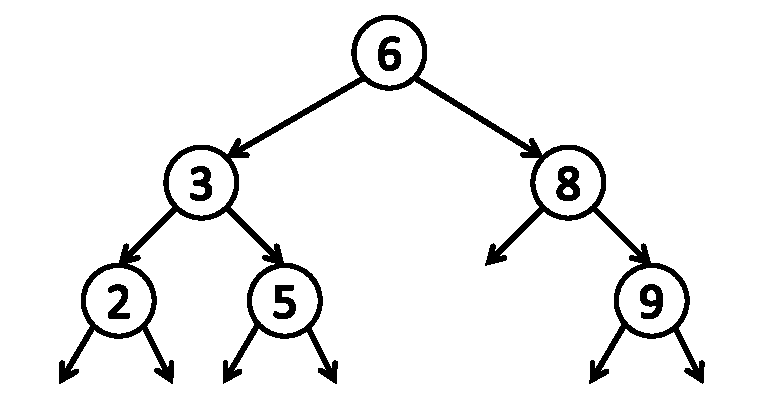
\includegraphics[width=0.5\textwidth]{figureTree.pdf}
%\caption{This is a figure text.}
%\label{fig:ex}
%\end{figure}
\newpage\
\pagestyle{empty}

\mbox{}

\pagebreak
\pagenumbering{roman}
\pagestyle{firststyle}
\textbf{\large{Abstract}}



With the increasing importance of big data processing, and the convergence of big data analytics and high performance computing, there is a need for new parallel computing frameworks and workflows that can process the 


\newpage
\textbf{\large{Acknowledgements}}

Acknowledgements goes here \lipsum[1]


\newpage
\tableofcontents
\pagebreak
\listoffigures
\pagebreak

\newpage
\pagenumbering{arabic}
\pagestyle{secondstyle}
\setcounter{page}{1}
\section{Introduction}


%  State of high performance computing
%  Shared memory and message passing
%  Role of different programming models/abstractions
%  Data centric computation
%  UPC++

%Scientific applications and engineering research are undergoing a transformation
%At the end of Dennard Scaling around 2004, transistor clock frequencies could not be raised without increasing the total circuit power consumption.
%Introduced multicore, manycore and accelerator-based computing 
%The big data revolution 
%Analysis, management, and collection of large volumes of data makes up the field of data-intensive science. 

%The core of high performance computing is writing efficient and parallel applications, which is the concern of researchers from an increasing range of disciplines, from physics and chemistry to medicine and geology. While the available hardware is being steadily improved,  \cite{engineering}. 


High performance computing is becoming of increased importance for scientists and researchers of a large range of disciplines, from physics and chemistry, to medicine and geology. At the very core of high performance computing lies the ability to write efficient and parallel software~\cite{engineering}.

The U.S department of Energy reported in 2013 through the Advanced Scientific Computing Advisory Subcommittee that the data volumes produced by scientific experiments and simulations were increasing more rapidly than the currently available algorithms, computing systems and workflows were able to keep up with. They also reported a need for innovations in high performance computing and data-intensive science to address challenges with contemporary systems related to concurrency, data movement, and energy efficiency~\cite{subcommittee}.

Big data frameworks such as Apache Hadoop~\cite{hadoop}, Spark~\cite{spark} and Flink~\cite{flink} can provide simple programming interfaces for distributed algorithms, with the underlying assumption that distribution of data and computing tasks can be handled by the system without programmer input. Programmers are given functionality to access data without explicitly managing communication between nodes. These systems are often reliant on coarse grained operations, which in many cases can produce inefficient programs, and limit the programmability of a framework~\cite{husky}\cite{piccolo}. Many data analytics operations are often orders of magnitude slower when implemented in a data analytics framework like Spark, than when written with native high performance computing tools such as MPI~\cite{bridgingthegap}. However, with a simple programming model, support for numerous data formats, underlying fault tolerance and automated data distribution, Spark remains an attractive option for distributed big data workloads~\cite{sparkacm}. 

As many scientific applications depend on processing high volumes of data, problems of high performance computing and big data analytics are converging. As the amounts of data increase, so does the importance of developing more efficient analytical tools~\cite{hpcabds}. Features from big data systems can be incorporated into HPC frameworks, to create programming models that are intuitive and higher-level, yet expressive and performant. This thesis presents Saddlebags, a framework that attempts to strike a balance between the two paradigms of parallel computing systems. Inspired by big data frameworks, Saddlebags support automatic distribution of data and computational tasks, and removes the need for specialized communication routines based on physical location. Inspired by HPC frameworks, Saddlebags allows fine grained memory access of distributed data, and leaves data movement during computations explicit and up to the programmer.

Saddlebags is implemented in C++. It uses parallelization and communication implementations from UPC++, a Partitioned Global Address Space library. With UPC++, a program has a static number of threads, each of which is given the affinity of a unique private memory segment. While data can be shared across segments, a memory segment is mainly accesses by the thread it has affinity to. Saddlebags applications can be used either on a single node or across multiple nodes within a compute cluster, using Ethernet or InfiniBand for network communication.

%while still allowing fine grained memory access, 


%Advantageous programming models from big data systems can be incorporated into 


%By incorporating concepts of simple programming models from big data systems, into HPC frameworks typically known for complex, we can develop tools that can solve problems that depend on both big data processing and performant computation.

%As the importance of advanced big data analytics

%Highly performant communication or computation a


%Designing efficient, yet intuitive programming models for distributed computing and data analytics seems to .

\subsection{Contributions}
A framework for implementing distributed algorithms and applications, created in and for C++, using UPC++, a library that provides PGAS mechanisms for communication. The framework provides an alternate programming model for distributed algorithms, in which a computational task, its data and its communication routines, is represented as a single object. 

% Distribution based on 


\subsection{Outline}
123

\newpage
\section{Background}
%  History + State of distributed computing / high performance computing
%  Message passing vs PGAS
%  Data intensive computing
%  Coupling of Data and processing task -> computation close to data
%  benefits of Abstractions + introduce data/task coupling as a potential 
%  Object oriented high performance computing: object contains data AND task
%  Distributed objects
%  
\subsection{State of High Performance Computing}
The field of high performance computing has experienced two major disruptions during the 21st century.

Software performance gains from increased frequency in single processing units reached its limits many years ago, and multi-core systems has been prominent in personal computing since. Up until the early 2000s, the speed at which computers could execute sequential programs would steadily increase as clock speed and semiconductor fabrication improved \cite{sutter_larus_2005}. Heat dissipation and energy consumption caused development of the maximum achievable CPU frequency to stall, effectively freezing the number of tasks that can be completed within a certain time frame on a single processing unit \cite{diaz_munoz-caro_nino_2012}. The answers to these problems were multi-core and many-core systems, which bypasses the aforementioned performance wall by utilizing several processing units.


Within the field of high performance computing, however, multi-processor systems were not a novelty. Using networks of workstation computers for parallel computation was an attractive alternative to traditional supercomputers, partly because new processor technology could easily be incorporated without replacing the entire system \cite{wilkinson_allen_2005}. While the field of parallel programming was relevant in high-end scientific applications before halt in clock speed development and the following \emph{concurrency revolution}, homogeneous distributed systems now dominate the field of high performance computing.


Multi-core and many-core architectures achieve parallelism through explicit task distribution and scheduling, managed by the programmer. Exploiting parallelism is often an application-specific issue, and can pose several challenges. In the fields of distributed- and high performance-computing, aiming for scalability further increases the complexity of the programming task. Several programming models have been devised to support development of distributed, parallel applications, and the current leading models can be clustered into different language paradigms: \emph{shared memory }and \emph{message passing} \cite{pgas_languages}. On top of these communication models, abstractions can be applied to hide complexity from the programmer in order to reduce development time and ease the debugging process. 

\subsection{Programming models}

There exists a perception that abstraction carry an inherent performance penalty, but abstractions can also be powerful tools in high performance computing \cite{mccandless_lumsdaine_1997}. For example, computing at a large scale can introduce issues relating to handling large amounts of data, scaling to a large or arbitrary number of computation nodes, or developing algorithms that utilizes communication routines and synchronization.

Identifying common patterns in different problems allows for development of frameworks and libraries that are optimized to handle classes of problems matching the same patterns. For example, the MapReduce framework hides significant programming overhead of problems that can be expressed within semantics provided by the framework and the programming model it represents. In its most primitive, data is supplied to the \emph{Map} function and a function to execute on the data is supplied to the \emph{Reduce} function. The MapReduce programming model is designed for algorithms and problems that can be expressed using these two functions, and the MapReduce framework is implemented to provide functionality that can be applied generally to problems within that programming model.

In addition to implementing communication routines and data distribution logic, a framework can supply scalability and fault tolerance, due to the information about the application that is implied by the programming model it is utilizing. Other examples of systems specialized in specific programming models include Dryad \cite{dryad}, which models an application's data flow into directed acyclic graphs, and Pregel \cite{pregel}, a framework for graph processing.

\subsection{Data intensive computing}



\subsection{Partitioned Global Address Space}
\cite{pgas_upc_energy}

Traditionally, parallel programming (and the field of High Performance Computing) has been clustered in two language paradigms: \emph{shared memory }and \emph{message passing} \cite{pgas_languages}.  Shared memory models provide an abstract memory space that is available for access across several concurrent compute threads. Message passing models, such as MPI \cite{MPI}, give a programmer control of the flow of execution by conceptually bundling most of the communication into a message abstraction. This approach can be used to achieve high performance; the programmer can reason about the cost of communication, and messages can be delivered between compute nodes to scale a program to large, multi-node systems.

Programming languages that achieve parallelism through a shared memory abstraction that provides memory access to several compute threads concurrently can be classified as Global Address Space (GAS) langauges. Communication between threads is achieved through reading and writing shared data, rather than explicit message passing \cite{gasnet_description}. Partitioned Global Address Space (PGAS) languages aim to provide a hybrid approach between previous parallelization paradigms, by utilizing the programmability advantages of the shared memory model, and the communication efficiency of message passing.

\subsubsection{GASNet}
GASNet is a communication API for GAS/PGAS languages that aims to provide a portable communication layer to systems that would otherwise be platform specific or network implementation dependent. Portability is achieved through translating PGAS programs to an intermediate C representation, which can be compiled into a platform specific application using the system's standard C compiler \cite{gasnet_description}.

GASNet is distributed with several API implementations with support for different underlying network architectures, called \emph{conduits} \cite{gasnetreadme}. This means that systems built on GASNet can be implemented to utilize different communication interfaces, including, among others, MPI, shared memory, UDP/IP, and InfiniBand verbs.

\subsection{Unified Parallel C}
Unified Parallel C, referred to as UPC, is a superset of the C programming language for writing SPMD programs, utilizing a global address space paradigm for parallelism. A complete UPC specification was first standardized in 2001, and several UPC compilers have been under development since, including GNU UPC, which is an extension of GCC \cite{web_gnu_upc}, and Berkeley UPC, which is dependent on GASNet \cite{web_berkeley_upc}.

The address space of a UPC program is partitioned into several logical fragments, with each concurrent thread being mapped to one fragment. With this model, each thread has affinity to its own individual memory region, which makes it possible to exploit data locality \cite{evaluation_of_upc} and utilize parallelism with the same language constructs.

Handling data in a memory partition mapped to a single thread makes it implicit that data is being accessed by a thread that has affinity to the given partition. Memory can also be explicitly distributed across several threads, using shared global memory, which disregards any thread affinity and is logically separated from the aforementioned thread-mapped memory partitions.

The shared memory abstraction of UPC is provided regardless of underlying hardware structure. Partitioned memory segments can be mapped to individual compute nodes in a cluster, utilizing data locality by performing computation on private data close to the location where it is stored, while still providing a shared memory abstraction for communication and programmability. The original UPC language specification states that a driving principle behind UPC is that parallelism and remote memory access should not obfuscate the resulting program; programmers should themselves utilize the language constructs to design programs and data structures, instead of being provided with solutions to specialized tasks. Additionally, the specification claims that a shared memory programming model is attractive for users of distributed memory systems \cite{upc_language_specification}. These two concepts can in part make up the motivation behind the UPC language.



\subsection{UPC++}
UPC++ is a PGAS extension to the C++ programming language. It is developed at University of California, Berkeley and saw the release of its 1.0 version in September 2017. UPC++ is implemented as a library extension, due to the complexity of developing a separate C++ compiler \cite{zheng_kamil_driscoll_shan_yelick_2014}. The library heavily utilizes C++ template programming \cite{web_cpp_template} for PGAS mechanisms, which allows the creation of library functions that use generic variables that can be adapted to different types. 

\subsubsection{Programming model}
UPC++ follows the SPMD model and like UPC utilizes threads with affinity to memory partitions. While UPC++ allows the use of C++ functionality such as objects and lambdas, it still aims to provide high performance and explicit communication by leaving much responsibility regarding concurrency and data movement to the programmer.

Each UPC++ partition has access to its own private memory segment, and is identified by its rank, an integer that can range from zero to the total number of partitions. Listing \ref{lst:helloworld} demonstrates a simple program that is started with 4 threads, each printing their rank, illustrating the Single Program Multiple Data property of UPC++ programs. Ranks can communicate through a logical shared memory segment, by utilizing UPC++ communication functionality, including global pointers, remote procedure calls (RPCs), and distributed objects. The number of ranks is static during execution; the total rank count is specified when launching a program and cannot be modified during runtime.


\begin{lstlisting}[label={lst:helloworld}, float, caption="Hello World"-program in UPC++ and its output, frame=tlrb, captionpos=b, language=c++, showstringspaces=false]
void main()
{
  upcxx::init();
  cout << "Hello world! " << upcxx::rank_me() << endl;
  upcxx::finalize();
}

-----------------------------------------------------------
Output:
Hello world! 0
Hello world! 2
Hello world! 3
Hello world! 1
\end{lstlisting}



Through communication or internal operations, a single thread may consist of several independent tasks that need access to computing resources for the program to continue its execution. In order to keep communication data movement predictable, a programmer will need to yield control of execution. This means that operations that require communication, such as RPC or global memory accesses, are separated from the main thread of execution and will not expend computing resources until explicitly granted permission to do so. Remote and asynchronous tasks are exposed to the caller through \emph{future} objects, which will change their internal state when the task has completed. This allows the caller to perform operations dependent on the completion of remote tasks or retrieval of remote data, and effectively communicate between ranks.

The 1.0 release of UPC++ introduced the concept of \emph{distributed objects}, which are objects defined by a generic type within UPC++ with the same identifier across all ranks. This means that data stored in the private memory segment of a partition can be referenced by a different rank in RPC calls. The data within the object is not implicitly distributed, but the name of the variable is. Local contents of the distributed objects can as such be explicitly distributed to any rank.

\subsubsection{Progress}
Outstanding asynchronous operations are not completed automatically, because the program consists of a static number of threads. In order to advance the internal state of UPC++ or complete RPC calls, computing resources are yielded from the main thread of execution via the \emph{progress()} function. This concept puts the responsibility of frequently progressing UPC++ state on the programmer's shoulders. The goal of this is to provide visibility of resource usage and parallelism, the latter being important to achieve interoperability with libraries and software packages that would otherwise restrict the use of multi-threading. Being cautious about where to progress RPCs relieves the needs for concurrency control such as mutexes, and implies atomicity in partition-internal operations of basic data types. More complex data structures that are not designed for concurrent access can be safely referenced in RPCs across partitions as long as the \emph{progress()} function is used only between atomic accesses.

\begin{lstlisting}[label={lst:distribobj}, float=t,frame=tlrb, caption={Communication through RPC, referencing a distributed object of an arbitrary C++ class. Rank 1 retrieves and prints \emph{myProperty} from rank 2's instance of \emph{myObj}.}, captionpos=b, language=c++, showstringspaces=false]
int main(int argc, char *argv[])
{
  upcxx::init();

  auto myObj = upcxx::dist_object<myClass>(myClass());
  upcxx::barrier();

  if(upcxx::rank_me() == 1)
  {
  
    auto f = upcxx::rpc(2, [](
      upcxx::dist_object<myClass> &my_dist_obj])
    {
      return (*my_dist_obj).myProperty;
    }, myObj);

    f.wait();
    std::cout << f.result() << std::endl;
    
  }

  upcxx::barrier();
  upcxx::finalize();
} 
\end{lstlisting}

\subsubsection{Remote Procedure Calls}

RPCs can be used for both modifying and copying data in the private segment of another rank's memory. The future objects returned by UPC++ RPCs can be used to indicate completion of the remote task, and communicate return values. A program that is dependent on data from a different rank, can halt advancement of the main thread by using the \emph{future.wait()} function, during which progress is attempted until the given future indicates that its corresponding remote operation has completed. This is not possible to achieve in tasks executed by progressing -- futures can only change state during progress, and progress-callbacks cannot themselves initiate further progress of other tasks. This concept provides a clear distinction between execution via the main thread of a rank, and execution via user-initiated progress of the same rank.

Listing \ref{lst:distribobj} demonstrates communication between two ranks using RPCs, distributed objects, and futures. A distributed object of an arbitrary class is initiated on all ranks, and a RPC is invoked to retrieve a property of the instance of the distributed object $myObj$ local to rank 2, back to rank 1. A barrier is used to ensure that the identifier of the distributed object is available on all ranks before it is referenced in the following RPC. The remote procedure is expressed with a lambda function, an unnamed function object. The RPC returns future $f$, which will hold a copy of the remote $myProperty$, the return value of the lambda function passed to the UPC++ $rpc$ function. The return value of the lambda will be available as \emph{f.result()} when the function has been executed, which is indicated by returning from \emph{f.wait()}. 

A distributed object is used in this example because it can be passed as a reference to the RPC on the sender's side, and it will be translated to the local copy of the distributed object with the same name on the receiving side. Non-distributed objects can only be passed as copy through RPCs, so distributed objects must be used for retrieving or modifying properties of remote objects. Within the RPC, the distributed object can be de-referenced to access properties of the underlying class. This is exemplified in listing \ref{lst:distribobj} through the access of $myProperty$.


\subsubsection{Global pointers}
Basic built-in C++ datatypes can be transmitted between partitions as RPC arguments or return values, by passing them as a copy. To communicate pointers to other partitions, the shared memory segment must be utilized. UPC++ can create a pointer to memory allocated in the shared memory segment, and copy local data to this location. The global pointer can be passed to other partitions through RPCs. Accessing global memory from a partition other than the one that initiated the pointer has to be done through asynchronous operations. UPC++ provides functions for remote puts and gets, which require internal progress on the partition that is hosting the shared memory in order to complete.

\newpage
\section{Design}
Saddlebags is a framework for parallel computing, aimed at applications and algorithms that can be implemented in C++. It uses UPC++ for thread spawning, communication, and data distribution, which provides PGAS mechanisms and language constructs such as remote procedure calls, virtual shared memory, and distributed objects. Saddlebags provides a programmer with objects and functions that are inherently distributed, and can be extended with methods and data to express different algorithms.

This section will cover the design and architecture of the system, outlining its different components, its programming model, and data flow. Section 3.1 explains the core concept and design philosophy of Saddlebags, Section 3.2 explains the programming model and data flow, while Section 3.3 outlines the architecture.

\subsection{Motivation}
Saddlebags is designed with several key features in mind, all of them related to what responsibilities a parallel computing framework can take off the an application developer's hands. Some of the underlying concepts and the motivation behind expanding upon the functionality of UPC++ follows.
\\


\hspace{4ex} \textbf{1. Computational tasks should be executed in the same partition in which the data it requires is located}

%TODO: CITATION FOR DATA PARALLELISM
Problems that can be expressed with data parallelism \cite{data_parallelism} can be distributed across computing units as individual tasks related to specific data. A key concept within PGAS programming is that a private memory segment has affinity to a single computing unit. To exploit data locality, a computational task should only be performed on the unit of computing which the data it requires has affinity to. Expressing behavior like this is trivial when the distribution of data is deterministic. Another wording of the same behavior is that computational tasks have affinity to the data it requires, the same way data has affinity to a computing unit and its private memory segment.
\\

\hspace{4ex} \textbf{2. A multitude of data should be implicitly distributed across available partitions}

Following the principle of a computational task's affinity to its data, full utilization of available processing units is only possible when a program's data is distributed. This means that data used in parallel processing should always be distributed across available memory partitions, so that the computational tasks that require the data is equally distributed.
\\	

\hspace{4ex} \textbf{3. The programmer should not need to write communication routines such as messages or remote procedure calls}

The purpose of building a framework on top of UPC++ is to provide interfaces for the implementation of distributed applications without the complexity of communication routines. While computation methods are application-specific, communication patterns can be implemented for a general case. When claiming that programmers are relieved of writing communication routines, it refers to the need for knowing where data is physically stored, which partition to communicate with, and the need for ensuring that messages are delivered before continuing computation. Data movement will still be explicit, but expressed in an abstraction level in which data locality and memory partitioning is not considered.

Saddlebags presents a programming model that is devised from a specific communication model, and it is assumed that algorithms that can be expressed within this model can also be implemented to communicate in a general pattern. Predictable communication patterns also allows for optimizations and reduces the need for application-specific synchronization. This also makes the physical distribution of data transparent to the programmer.
\\

The goal of building a framework on these specific features is to allow computational parallelism to be expressed with the same semantics as data parallelism, while still allowing tasks to communicate data between each other. The complexity of implementing applications that fit this classification is reduced by utilizing a general communication pattern that relieves programmers of implementing specialized communication. Programmers will in this framework use communication routines by referring to data rather than physical location in the form of partition or computing unit.

\subsection{Programming model}
The programming model and data flow model of Saddlebags is based around coupling data and functionality together into an object. Objects that serve the purpose of executing computational tasks in Saddlebags are named \emph{Items}. Items contain pre-existing general communication methods, and the main effort of developing an application with Saddlebags is implementing the computational tasks within an item, and integrating communication and data-flow into that task.

Items of different types can be implemented in the same application, and stored in different \emph{tables}. The behavior of tables cannot be extended by the programmer, but every application must define their tables by name and item type. Tables are common for every partition, while an instance and name of an item can only exist on a single partition. This is how distribution of data is achieved: items are spread across partitions, while the tables that contain them exist on every partition, and can reference items regardless of physical location.

\begin{figure}[h]
\centering
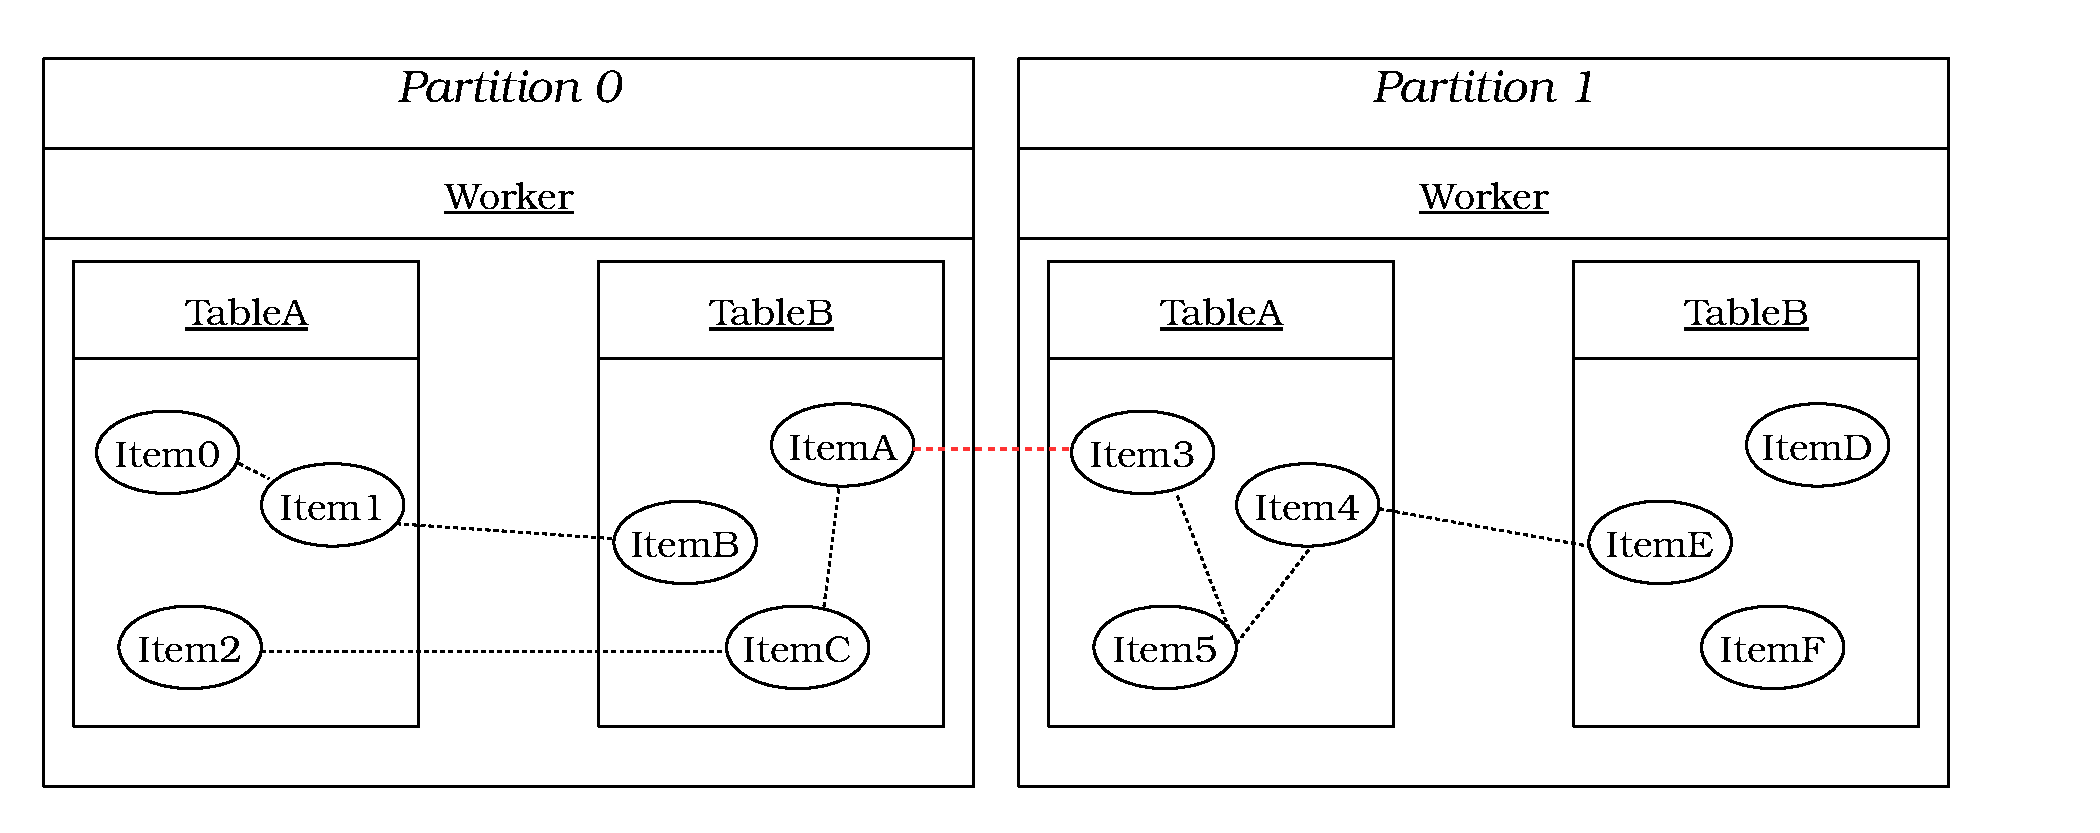
\includegraphics[width=16cm]{illustrations/basicmodel.pdf}
\caption{Overview of the key data structures in a Saddlebags application.}
\label{fig:basicmodel}
\end{figure}

The relation between items, tables and partitions are illustrated in figure \ref{fig:basicmodel}. This illustration shows a basic design of a Saddlebags application with two tables and two UPC++ partitions. Underlined names are objects that exist on every partition. Lines indicate example communication, with red lines indicating communication between different partitions. Items of different types are stored in different tables, and the same tables are available on both partitions. Item names are unique across all partitions, and a single item have affinity to a single partition. 

Tables are stored within a \emph{worker}, a distributed object. Tables are referenced via this object. The behavior of the worker need not be extended by the programmer, and in the context of data flow and execution model the worker is relatively insignificant, and will be mostly ignored in this section. It will be explained further when discussing implementation and interoperability with UPC++.

Items implement a \emph{work-push-pull} model, in which \emph{work} refers to a computational task implemented in the item class, and \emph{push} and \emph{pull} are the two available modes of communication. The work of an item is designed to be executed iteratively, and each iteration of a Saddlebags application involves executing work and performing any communication routines that was called as a result of the work. An iteration applies to every item in every table, and it is with this iterative model that an application can be executed. 

\subsubsection{Events}
The data flow model of Saddlebags is implemented with the concept of \emph{events}. Within the context of this framework, an event refers to the receiving of any communication message, or reaching specific points of the iteration process. Whenever an event is triggered, for example when receiving a \emph{pull} message, the item that received the message calls a corresponding method, in this case a \emph{foreign pull} method. The contents of this method can be implemented differently in different item types, and it is also able to initiate other communication routines. This is directly related to the data flow of an application: when receiving a pull event, the event-triggered method determines what data to return. When the message returns to the original sender with some data, event-triggered return method determines how to handle the data. 

\begin{table}
\setlength\arrayrulewidth{1pt}
\renewcommand{\arraystretch}{2}
\begin{tabular}{ | p{3cm} | p{6cm} | p{6cm} |}
   	\hline
   	\textbf{Method} & \textbf{Event} & \textbf{Implied data movement} \\ \hline
   	On Create & Item is created & None\\ \hline
  	Refresh & An item with the same name is attempted created & None \\ \hline
  	Work & Start of iteration & None \\ \hline
   	Foreign Push & A push message is received from another item & Data from sender is received with the message  \\ \hline
   	Foreign Pull & A pull message is received from another item & Return data is sent back to the sender\\ \hline
	Returning Pull & A pull message that originated in this item has returned & Data from pull target is received with the message\\ \hline
	Finishing Work & End of iteration & None\\ \hline

\end{tabular}
\caption{All events and their corresponding methods}
\label{table:events}
\end{table}

Table \ref{table:events} lists all methods in the item class that can be triggered by events. Column 1 lists the names of the methods, column 2 lists the circumstances under which the method is called, and column 3 lists what data is moved in the corresponding method. All methods with data movement is called as a result of communication with other items. Communication routines can be initiated in any of the methods listed in the table. Items are referenced by name, so two items with the same name cannot exist in the same table. The \emph{Refresh} method is used to incorporate this behavior in a program.
\\ \\
\subsubsection{Example}
The programming model that is implied by items and events can be explained further through an example application. Consider the PageRank algorithm, a mathematical expression for ranking the importance of a website \cite{pagerank}. The following expression is a simplified way of calculating the Page Rank ($PR$) of a website ($u$), given a list of pages that link to it ($B_u$), and the total number of links from those websites ($N$):

\vspace{10pt}
\begin{center}
${\displaystyle PR(u)=\sum_{v\in B_{u}}{\frac{PR(v)}{N(v)}}}$

\end{center}
\vspace{20pt}

It is assumed that every page starts with a PageRank of 1. Given a list of pages and their outgoing links, a PageRank application can be designed with the Saddlebags programming model. Each page is implemented as an item, and each item is given a list of its own outgoing pages, in addition to a PageRank value and a buffer for calculating a new PageRank, set to 0. Only one table and one type of item is needed. The required methods are listed in table \ref{table:pagerankevents}. When the items are created, the algorithm can be ran for as many iterations of PageRank as needed, since one PageRank iteration (one execution of the aforelisted formula for each item) is equivalent to one Saddlebags iteration.

\begin{table}[b]
	\setlength\arrayrulewidth{1pt}
	\renewcommand{\arraystretch}{2}
	\begin{tabular}{ | p{3cm} | p{12cm} |}
		\hline
		\textbf{Method} & \textbf{Functionality} \\ \hline
		Work & Each page that this item links to will receive a push message with this item's PageRank divided by this item's count of outgoing links \\ \hline
		Foreign Push & Add the incoming value to the new PageRank buffer \\ \hline
		Finishing Work & PageRank of this item is set to the value of the buffer. The buffer is set to 0.\\ \hline
		
	\end{tabular}
	\caption{The methods required to implement PageRank with Saddlebags}
	\label{table:pagerankevents}
\end{table}

\subsection{Architecture}
Programming a Saddlebags application involves two main tasks: extending item methods to fit a computational purpose, and creating items through data input. In the example illustrated in the previous section, table \ref{table:pagerankevents} shows the extension of an item, and feeding outgoing links to an item is an example of data input. Items are referred to by the name of the table that contains it, and the name of the item itself. Tables are initialized with a name, and an item type, which also means that each table can only contain items of a single type. 



\subsubsection{Item}


\subsubsection{Table}
Distributor

The communication patterns of a push/pull paradigm is simple enough that the cost of data movement as a result of communication in an application can be reasoned about, despite implementation complexity being hidden. 

Saddlebags is designed with the goal that abstractions provided by the programming model, through C++ mechanisms such as inheritance and type templates, should not affect algorithmic complexity. This will likely only be true for algorithms that can be tailored to the push/pull/work paradigm. 


\newpage
\section{Related work}
\subsection{Husky}
\subsection{Spark}
\subsection{DataMPI}
\subsection{Legion}
%% Data MPI?
%% PGAS energy evaluation?

\newpage
\section{Implementation}
\subsection{Overview}
\begin{figure}[h]
	\centering
	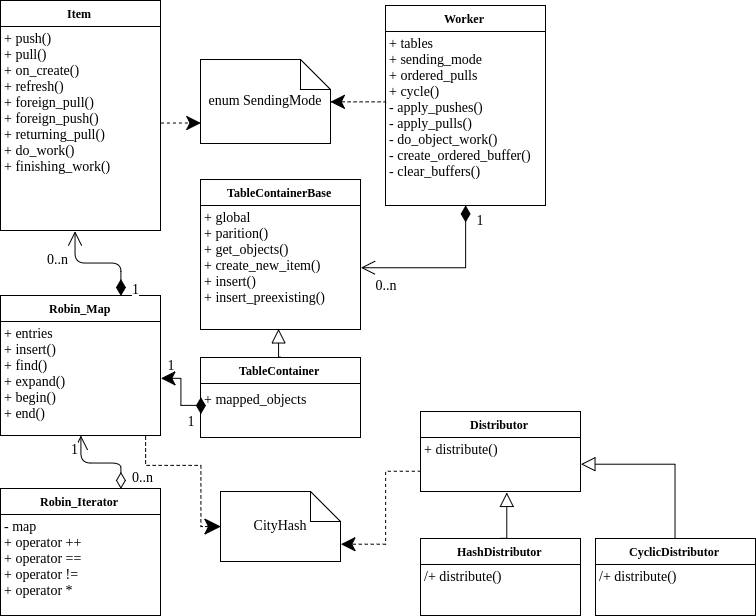
\includegraphics[width=16cm]{illustrations/uml.png}
	\caption{UML diagram of Saddlebags' main classes.}
	\label{fig:uml}
\end{figure}



\subsection{Distributed objects}

\subsection{Templates}
\subsection{Table}
\subsection{Communication}
%message
\subsection{Synchronization}
%barriers in cycle
\subsection{Usage}

\newpage
\section{Evaluation}
\subsection{Expressiveness}
\subsection{Energy efficiency}
\subsection{Abstraction costs}
\subsection{Comparison with other systems}

\newpage
\section{Discussion}
%other features from spark

\newpage
\section{Future work}
\subsection{Fault tolerance}
\subsection{View based serialization}
\subsection{File input}

\newpage
\section{Conclusion}




\pagebreak
\bibliographystyle{ieeetr}
\bibliography{report}

% End of document
\end{document}
\grid
\grid
